%----------------------------------------------------------------------------
\appendix
%----------------------------------------------------------------------------
\chapter*{\melleklet}\addcontentsline{toc}{chapter}{\melleklet}
%----------------------------------------------------------------------------
\setcounter{chapter}{13} % M betű
\setcounter{section}{0}
%\setcounter{equation}{0}
\numberwithin{equation}{section}
\numberwithin{figure}{section}
\numberwithin{lstlisting}{section}
%\numberwithin{tabular}{section}

%----------------------------------------------------------------------------
\section{Első melléklet}
%----------------------------------------------------------------------------

A melléklet(ek)ben olyan információkat célszerű elhelyezni, melyek nélkül a 
főszövegben közöltek nem értelmezhetők, de az ott történő elhelyezésük 
jelentősen megnövelné a főszöveg terjedelmét. A mellékletbe kerülnek például a

\begin{itemize}
  \item terjedelmes, sok adatot tartalmazó táblázatok,
  \item mérési és egyéb jegyzőkönyvek,
  \item levél és faxmásolatok,
  \item szerződésmásolatok,
  \item műszaki rajzok és műszaki leírások,
  \item nagyméretű, ill. összetett kapcsolási vázlatok,
  \item térképek,
  \item fényképek. 
\end{itemize}

A mellékletbe kerülő információ mennyisége esetenként szükségessé teheti több 
melléklet kialakítását. Ebben az esetben célszerű lehet azt például a fenti 
csoportosításban kialakítani, és az egyes mellékleteket folyószámmal ellátni 
(1. Melléklet, 2. Melléklet stb.). 
Az első melléklet új páratlan, a többi új oldalra kerüljön. 
A melléklet tipográfiai kialakítására ugyanazok a szabályok vonatkoznak mint a 
függelékére. 
Minden, a mellékletben található információhordozót (táblázat, ábra, 
fénykép stb.) egyedi számmal és címmel kell ellátni. Ezt az azonosítót kell 
használni a főszövegben az ezekre való hivatkozások során.

\begin{figure}[!ht]
\centering
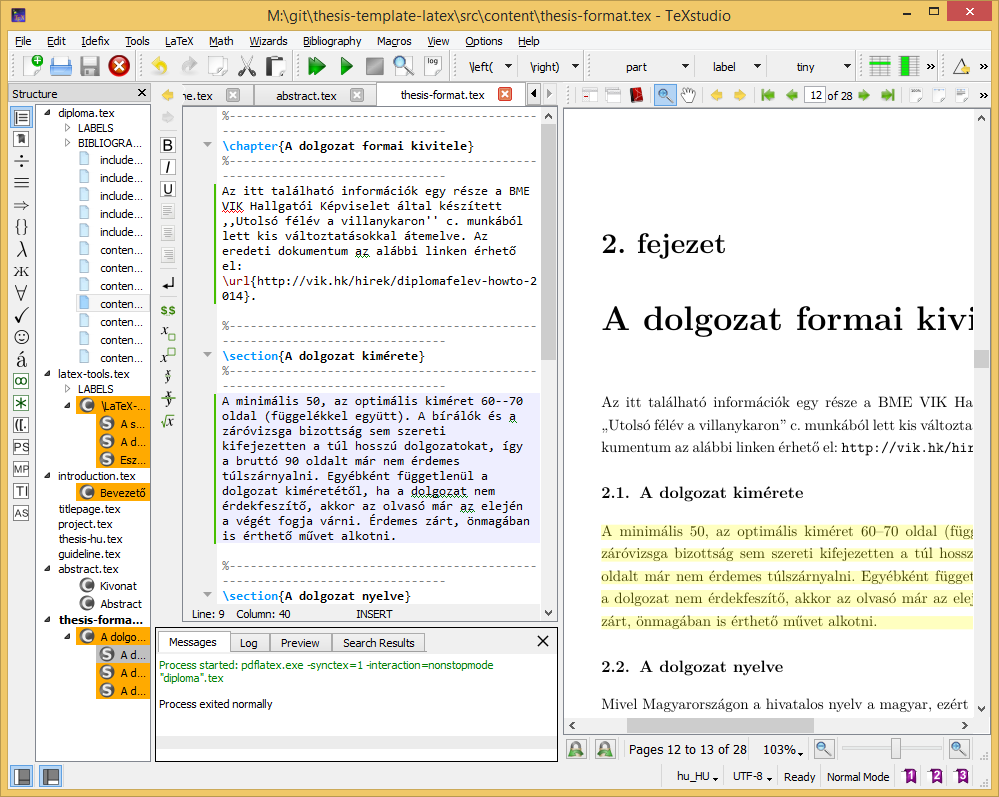
\includegraphics[width=50mm, keepaspectratio]{figures/TeXstudio.png}
\caption{A TeXstudio \LaTeX-szerkesztő.} 
\end{figure}


%----------------------------------------------------------------------------
\clearpage
\section{Kapcsolási rajzok}
%----------------------------------------------------------------------------

% Képfelirattal ellátott kapcsolási rajzok, táblázatok, fényképek...
